\chapter{Introduction} \label{chap:intro}

Over the last decade, Software development had a tremendous impact with increasing customer demand and requirements \cite{article:swdemand:ahmed}. 
So, the developers have come up with different techniques to meet this requirement criteria. 
Similarly, increasing product complexity and ambiguity have a significant impact on software development. 
Early user feedback from potential customers in the industry is crucial for creating successful software products because of the growing market uncertainties, and consumers' desire to receive integrated solutions to their issues rather than unique software developments \cite{misc:businessmodels:teece}.
With the increasing complexity of products, it becomes challenging to determine user requirements.
Different people can have overlapping or contradicting opinions. 
And to reduce these risks, there has to be early detection of the user's needs and requirements. 
Giving users a ``partially functioning'' system is the most excellent method to determine their requirements \cite{journal:prototyping:davis}.
This ensures that the developers with high uncertainties in the early product development can validate by testing the underlying assumptions \cite{misc:lean:steve}.

Developers can use this feedback to validate the most critical assumptions about the software product. 
This validation can be used to decide whether to add, remove or update a feature \cite{article:experiments:lindgren}. 
This process is called \texttt{Continuous Experimentation (CE)}.
There has been an increase in interest in the types of experimentation that can take place in product development. 
Fabijan et al. \cite{paper:controlled: experiments} have shown the benefits of continuous experiments in many use cases with incremental product improvement. 
In CE, the product owner designs different software variants (E.g., Different Subscription fees for registration) of the product, and the developer integrates these variants and assigns them to a distinct group of users. The variant with better results as per some evaluation criteria (more number of user registrations) is deployed for the entire set of users.
So, an experiment can be valuable when it solves real-world problems.
Hence, for experiments to be successful, they should offer one or more solutions that will benefit users.
The developers are responsible for creating the experiments, and the Product owners give the ideas and feedback. 
This created a problem of a gap between the developers and the product owners and raised a question of how the product owners can be closely associated with the developers.

To solve this problem, the developers focus more on automating the software code rather than coding everything stated in the product requirements \cite{article:prototyping:hoffnagle}.
This approach is formally known as a \texttt{Low-code} or \texttt{No-code} approach.
So, this approach helps to have a UI interface for the non-developers to understand and develop the software products \cite{paper:lowcode:khorram}.
One approach to support the product owners in developing the variants is UI Prototyping. 
UI prototyping creates new UI variants using predefined UI elements (E.g., Drag and drop the UI elements into the screen). 
This helps product owners to be creative and innovative because it gives them visual feedback.
So, if UI prototypes are developed in a low-code technique, they would be lightweight software.
This helps the product owner develop various prototypes and conduct experiments on the users.
Similarly, it would save a lot of resources and, at the same time, get feedback from the users.

According to Luqi et al. \cite{paper:prototyping:luqi}, Models are used broadly in prototyping because a model represents or describes the aspects of the systems that cannot be described adequately in a system of interest.
Modeling the system is far more convenient and efficient than the actual development process. 
Moderately accurate models can be created using an iterative approach in software development by getting continuous feedback from the users.

Most often, data is used to measure the success of the experiments by getting significant feedback from the users.
Promising experiments are designed to better some goal or metric. 
A worthwhile product experiment's ``secret ingredient'' is meaningful, actionable consumer feedback regarding the effects of your product experiments.
This can be done using the \texttt{Qualitative and Quantitative} data analysis.
Using a combination of qualitative and quantitative data can improve an evaluation by ensuring that the strengths of another balance the limitations of one type of data.
This will ensure that the knowledge is improved by integrating different ways of understanding.
\begin{figure}[ht]
    \centering
    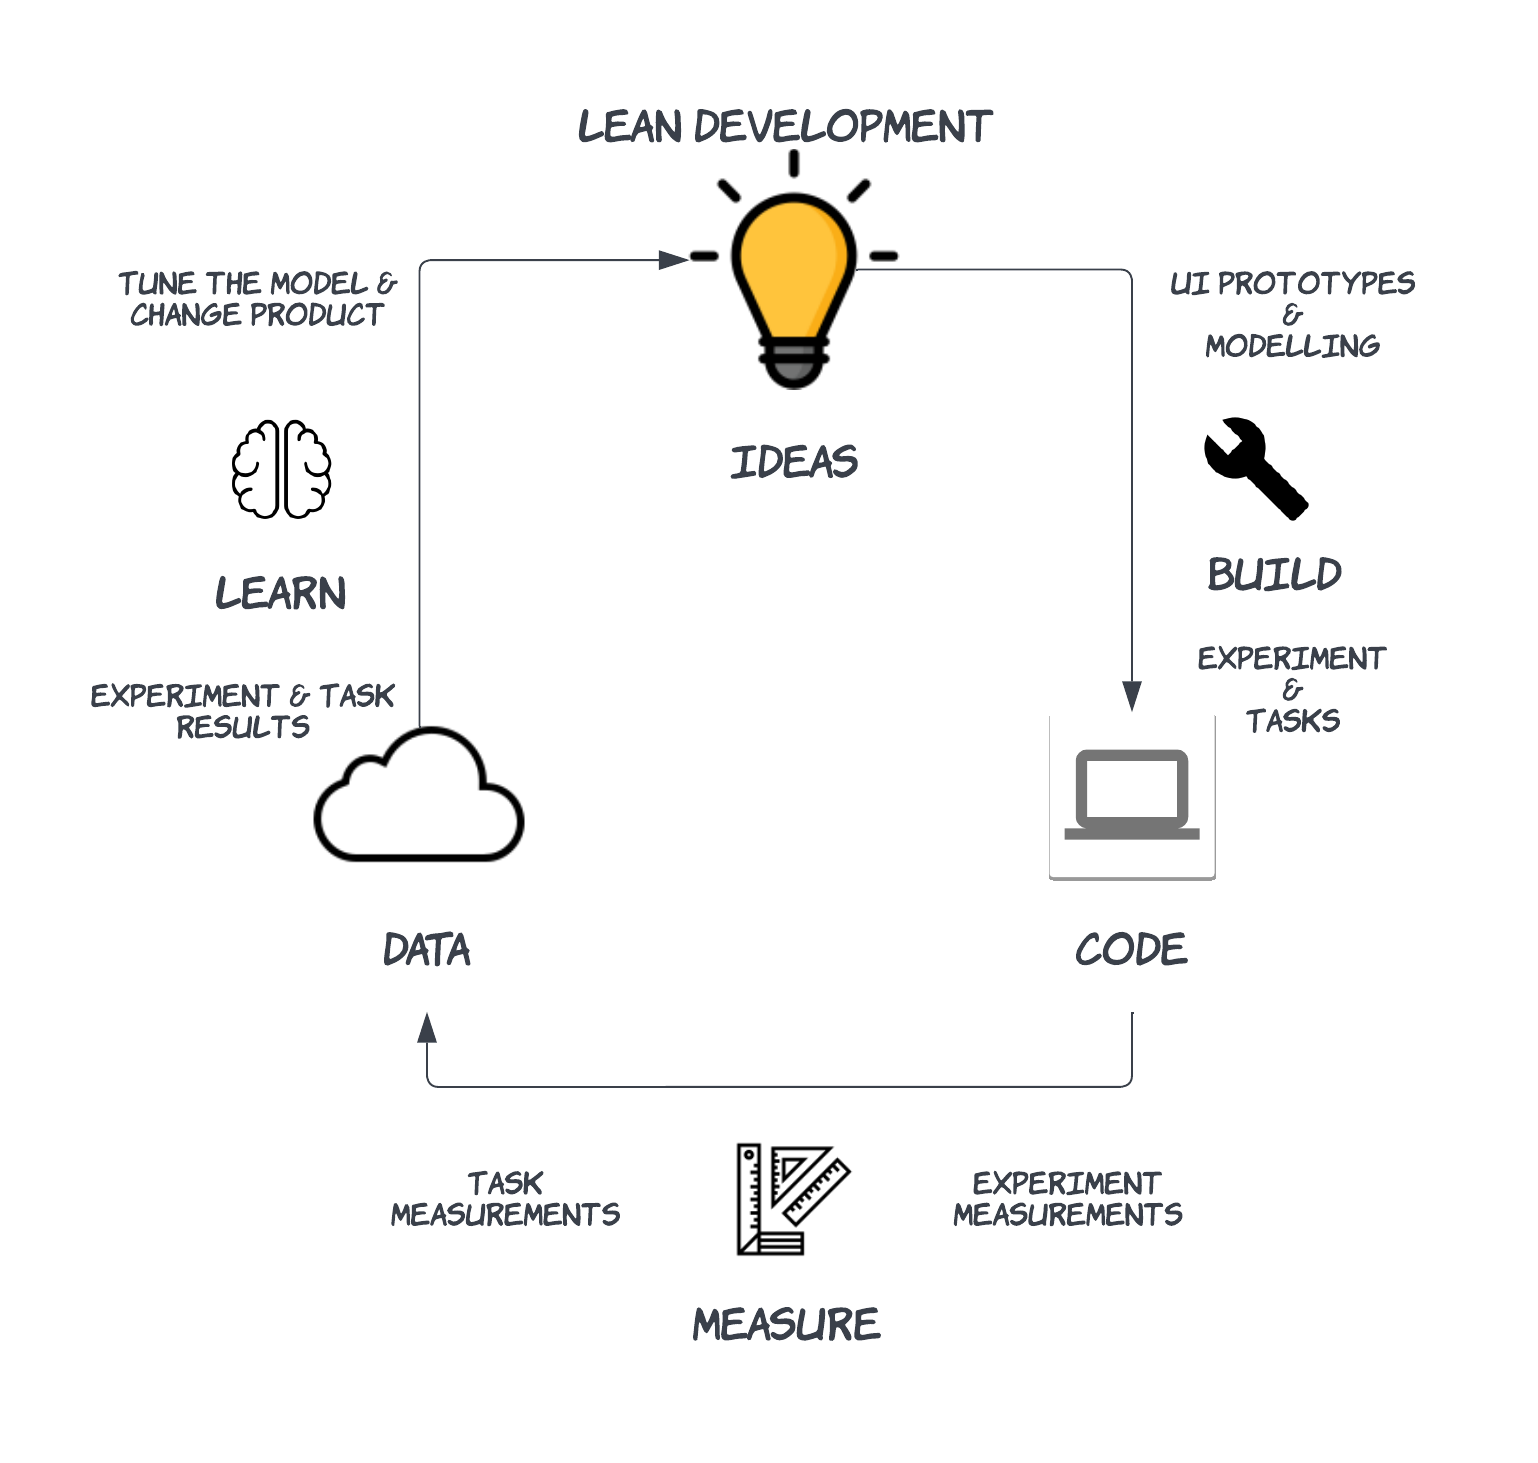
\includegraphics[scale=0.22]{images/solution-ideas/LEAN.png}
    \caption{LEAN Development technique}
    \label{intro:fig:lean}
\end{figure}
\par
In our solution, we propose to combine the Crowdsourcing Design principles (DP) \cite{misc:crowdsourcing:sg} with model-based and data-driven approaches to solve the problems faced by product owners and developers to have a successful software product.
For that, we use the \emph{LEAN} development technique (see figure \ref{intro:fig:lean}) by starting with \texttt{(1) Ideation and Creating UI prototypes}, then \texttt{(2) Building the product by developing the Models} and using the \texttt{Low-Code technique}, \texttt{(3) Create Experiments} to have a UI for the users and get feedback from the users and finally \texttt{(4) Analyze the data and Tune the model}.